\chapter{LLVM}
\section{History}
The \llvm is a collection of modular and reusable compiler and tool chain technologies to support static and dynamic compilation as well as transparent and lifelong program analysis and transformations of arbitrary programs \cite{LLVMWebsite, LLVMResearchBeginning}.\\
The main goal of \llvm consists of the creation of a compiler framework in which the optimizations and analysis are independent from the underlying OS and the used programming language.
To archive the independence \llvmir was introduced which is solely used within the pipeline.
\enquote{\llvmir is a strongly typed, \ac{SSA} language that connects to a wide variety of high-level languages} \cite{PolyhedralEmpiricalStudy}.\\
Originally \llvm has been a research project, which was first described in a publication in 2004, at the university of Illinois.
Since that the project has grown so popular that in 2014 the LLVM Foundation was founded for organizing and maintaining the project \cite{LLVMFoundation}.\\

\section{Pipeline}
When entering the pipeline of \llvm (\autoref{fig:llvmPipeline}) the \llvmir putting the independence from the programming language into effect is generated by translating the files containing source code written in an arbitrary programming language using a frontend like clang \cite{clang}.
When leaving the pipeline files containing the appropriate assembler instructions are created out of the (possibly) newly formed \llvmir \cite{IntroLLVM}.
\begin{figure}[!ht]
    \caption[A possible pipeline of LLVM]{
        This visualizes a possible pipeline of \llvm.
        The reason for a \enquote{possible} pipeline is that the \linker is not necessary when only operating on a single \llvmir file.\tikzlegend
    }
    \label{fig:llvmPipeline}
    \centering
    \begin{tikzpicture}
        \node(languages)[nonLlvmIrNode, align=center]{C/C++, Obj-C,\\Python, Ruby,...};
        \node(frontend)[nonLlvmIrNode, right=of languages, align=center]{compiler\\frontend};
        \node(opt1)[llvmIrNode, right=of frontend]{\opt};
        \node(llvmLinker)[llvmIrNode, below=of opt1]{\linker};
        \node(opt2)[llvmIrNode, below=of llvmLinker]{\opt};
        \node(generator)[llvmIrNode, left=of opt2, align=center]{LLVM Code\\Generator};
        \node(linker)[nonLlvmIrNode, left=of generator]{System Linker};
        \path[nonLlvmIrPath] (languages) to (frontend);
        \path[llvmIrPath] (frontend) to (opt1);
        \path[llvmIrPath] (opt1) -| ($(opt1.north east) + (0.5,0.5)$) -| node[auto, above=0.1cm, left=0.1cm]{Pass} (opt1);
        \path[llvmIrPath] (opt2) -| ($(opt2.south east) + (0.5,-0.5)$) -| node[auto]{Pass} (opt2);
        \path[llvmIrPath] (opt1) to node[auto, swap]{Multiple files} (llvmLinker);
        \path[llvmIrPath] (llvmLinker) to node[auto, swap]{Single file} (opt2);
        \path[llvmIrPath] (opt2) to (generator);
        \path[nonLlvmIrPath] (generator) to (linker);
    \end{tikzpicture}
\end{figure}
\subsection{compiler frontend}\label{subsec:compilerfrontend}
The first step of the pipeline is translating the files containing sourcecode by a front end like clang (C, C++, Objective-C), flang (Fortran) \cite{fortranllvm}, llvm-ruby (Ruby) \cite{rubyllvm}, PyLLVM (Python) \cite{pyllvm}, llvm-lua (LUA) \cite{luallvm} and can be further extended to all languages GCC supports by using dragonegg \cite{dragonegg} which replaces the optimizer and code generators of GCC by the ones of \llvm.
From now on this work is only discussing clang as frontend.
This study is working on C/C++ so only clang is used.
Using clang \llvmir can be generated by adding the option \texttt{-emit-llvm} in order \enquote{to abstract away from the specifics} \cite{FastScopDetection} of a programming language.
The option \texttt{-S} may also be passed to generate a human readable text file instead of a \llvmir binary.
\subsection{LLVM Optimizer}\label{subsec:optimizer}
On files containing \llvmir the \opt can perform steps for optimizing and analyzing the code.
These steps are called \enquote{passes}.
Such passes can be invoked explicitly by appending the appropriate options to the command \texttt{opt} of the the \opt and are applied either to single files or to the already linked program.
It is also possible to add further custom options by loading (multiple) libraries using the flag \texttt{-load}.
When calling the \opt the option \texttt{-S} may also be specified for generating a human readable text file similar to clang in \autoref{subsec:compilerfrontend}.
\subsection{LLVM Linker}
The \linker is an optional step which is not necessary when operating only on a single \llvmir file.
But when operating on multiple files the \linker links the optimized \llvmir files into a single \llvmir file and applies further optimizations at link time.
\subsection{LLVM Code Generator}
When all desired passes are performed the \generator translates \llvmir into target assembler.
\subsection{Basic Blocks}\label{subsec:basicBlock}
The underlying structure the pipeline is working on are basic blocks.
According to \cite[chapter 8.4, p.~525]{Drachenbuch} basic blocks
\begin{comment}
    Seite 525, Chapter 8. Code Generation, 8.4 Basic Blocks and Flow Graphs
\end{comment}
\begin{quotation}\noindent
    \grqq[...] are maximal sequences of consecutive three-address instructions with the properties that
    \begin{enumerate}[label=(\alph*)]
        \item The flow of control can only enter the basic block through the first instruction in the block.
        \item Control will leave the block without halting or branching, except possibly at the last instruction in the block.\grqq
    \end{enumerate}
\end{quotation}
\subsection{Control Flow Graph (CFG)}\label{subsec:cfg}
The \cfg is a representation of the connections between basic blocks called control flow \cite[chapter 8.4.3, p.~529]{Drachenbuch}.
\begin{comment}
    Seite 529, Chapter 8. Code Generation, 8.4.3 Flow Graphs
\end{comment}
\begin{quotation}\noindent
    \grqq The nodes of the flow graph are the basic blocks.
    There is an edge from block \(B\) to block \(C\) if and only if it is possible for the first instruction in block \(C\) to immediately follow the last instruction in block \(B\).
    There are two ways that such an edge could be justified:
    \begin{itemize}
        \item There is a conditional or unconditional jump from the end of \(B\) to the beginning of \(C\).
        \item \(C\) immediately follows \(B\) in the original order of the three-address instructions, and \(B\) does not end in an unconditional jump.\grqq
    \end{itemize}
\end{quotation}
\begin{code}
    \caption[Source of matmul.cpp]{The source of matmul.cpp represents a kind of matrix multiplication which is blotched with calls to \texttt{rand(...)} in order to break some \scops (see \autoref{subsec:definitionScop}) and make it slightly more interesting for investigation.}
    \inputminted{c++}{cpp/matmul.cpp}
    \label{lst:matmulcpp}
\end{code}
\begin{figure}[!h]
    \caption[The CFG of \autoref{lst:matmulcpp}]{
        This figure contains the \cfg of \autoref{lst:matmulcpp}.
        It visualizes the connections of the basic blocks (see \autoref{subsec:basicBlock}).
        Every loop of the five within \autoref{lst:matmulcpp} consists out of four basic block which are typically called \texttt{for.condX} (Deciding whether to perform a further iteration or not), \texttt{for.bodyX} (Part of the loop body to execute), \texttt{for.incX} (Increment the iteration variable) and \texttt{for.endX} (The block called when leaving the loop) where \texttt{X} is a placeholder for an optional number.
        When using a release build of \llvm these names are stripped and replaced by simple numbers.
    }
    \label{fig:exampleCfg}
    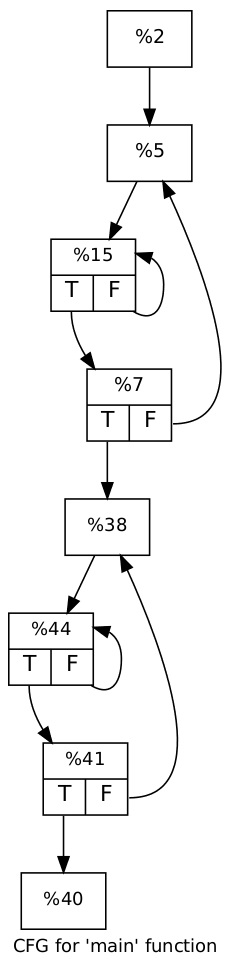
\includegraphics[width=\textwidth]{gfx/matmulCfg.png}
\end{figure}
Therefore the \cfg is very important to the pipeline as it is needed by many analysis and optimization passes to determine whether certain optimizations can be applied and in which way.
The current \cfg of a \llvmir file can be generated at any point of the pipeline.
It also can be visualized (like \autoref{fig:exampleCfg}) by passing one of the options \texttt{-view-cfg} or \texttt{-view-cfg-only} to the \opt.
\begin{enumerate}
    \item Translate the C++ sourcecode of \autoref{lst:matmulcpp} into \llvmir (\autoref{lst:matmulll})\\
        \texttt{clang++ -S -emit-llvm matmul.cpp -o matmul.ll}
    \item Generate the \cfg\\
        \texttt{opt -view-cfg-only matmul.ll}
\end{enumerate}
